\chapter{Financial Model: 12--24 Month Extension}
\label{ch:financial-model}

\section{Source map: every number traceable}

Three workbooks exist and disagree by design --- they are successive realism passes, not three live scenarios.

\begin{table}[htbp]
\centering
\caption{Source workbooks and their status}
\label{tab:source-workbooks}
\small
\begin{tabular}{p{3.4cm}p{5.6cm}p{4.0cm}}
\toprule
\textbf{Workbook} & \textbf{What it models} & \textbf{Status} \\
\midrule
\texttt{devorix-financial-\allowbreak model.xlsx} & Original aggressive ramp (500\(\to\)100,000 devs/12mo, fill 2\%\(\to\)55\%, \$2 eCPM) & \textbf{Superseded.} Stale \textrm{\textrupee}86 FX, CPM-only model that MASTER-PLAN \S 5 overrides. Kept only for the steady-state sensitivity table (Section~\ref{sec:unit-economics}). \\
\texttt{devorix-financial-\allowbreak model-REALISTIC.xlsx} & Grounded 4-month plan: \(\leq\) 500 installs, flat sponsorship deals, \textrm{\textrupee}94.5 FX & \textbf{Base case for Months 1--4.} Matches MASTER-PLAN \S 8.3 to the rupee. \\
\texttt{devorix-financial-\allowbreak model-v3-TIMEBASED.xlsx} & Same plan on a time-based (hours-coding \(\times\) \%-wait) impression count, plus a Global/Blended scenario & Used for impression mechanics, global sensitivity, and implied-eCPM cross-check. \\
\bottomrule
\end{tabular}
\end{table}

\textbf{Months 1--4 are not modeled here --- they are locked, audited inputs} that agree across MASTER-PLAN \S 8.3 and both current workbooks to the rupee \cite{masterplan_2026}.

\section{The honest stage framing}

Pre-launch, pre-revenue, 0 advertisers, 0 installs, solo founder, \textrm{\textrupee}1 lakh budget. \textbf{Founder salary is modeled at \textrm{\textrupee}0 (sweat equity)} --- these are not fully-loaded costs and exclude founder opportunity cost entirely; investors should read margins with that in mind. Everything past Month 4 is gated on MASTER-PLAN \S 8.3's go/no-go test (\(\geq\) 2 advertisers paid \emph{and} renewed, week-4 retention holds, founder still wants to run it). The 12--24 month curves are \textbf{planning scaffolding, not a funded forecast}.

\section{Months 1--4: locked base case}
\label{sec:months-1-4}

\begin{table}[htbp]
\centering
\caption{Months 1--4 locked base case (audited, not modeled)}
\label{tab:months-1-4}
\small
\begin{tabular}{lrrrrl}
\toprule
\textbf{Metric} & \textbf{M1} & \textbf{M2} & \textbf{M3} & \textbf{M4} & \textbf{Source / Label} \\
\midrule
Installs (cumulative) & 100 & 250 & 400 & 500 & \textit{Verified (locked input)} \\
Active devs (WAU 40\%) & 40 & 100 & 160 & 200 & Same \\
Advertisers (flat deals) & 1 & 2 & 2 & 3 & Same \\
Revenue (\textrm{\textrupee}) & 15,000 & 30,000 & 30,000 & 45,000 & Same \\
Dev payout pool (\textrm{\textrupee}, 50\%) & 7,500 & 15,000 & 15,000 & 22,500 & Same \\
Fixed costs (\textrm{\textrupee}) & 5,060 & 5,120 & 5,120 & 5,180 & infra \textrm{\textrupee}3,000 + misc \textrm{\textrupee}2,000 + payout txn \\
Net profit (\textrm{\textrupee}) & 2,440 & 9,880 & 9,880 & 17,320 & Same \\
\textbf{Cumulative net (\textrm{\textrupee})} & 2,440 & 12,320 & 22,200 & \textbf{39,520} & Matches MASTER-PLAN \S 8.3's ``\textasciitilde 39,500'' \\
Implied eCPM (\textrm{\textrupee}/1,000 views, v3) & 19.7 & 15.8 & 9.9 & 11.8 & Flat-fee underprices impressions as audience grows \\
\bottomrule
\end{tabular}
\end{table}

\begin{figure}[htbp]
\centering
\begin{tikzpicture}[
  every node/.style={font=\small},
  box/.style={draw, rectangle, minimum width=3.0cm, minimum height=1.0cm, align=center},
  neg/.style={draw, rectangle, minimum width=3.0cm, minimum height=1.0cm, align=center, fill=red!15},
  posbox/.style={draw, rectangle, minimum width=3.0cm, minimum height=1.0cm, align=center, fill=green!15}
]
\node[box, fill=blue!15] (rev) at (0,0) {Revenue\\ \textrm{\textrupee}45,000};
\node[neg, right=1.2cm of rev] (payout) {Dev payout\\ \(-\)\textrm{\textrupee}22,500};
\node[neg, right=1.2cm of payout] (fixed) {Fixed costs\\ \(-\)\textrm{\textrupee}5,180};
\node[posbox, right=1.2cm of fixed] (net) {Net\\ \textrm{\textrupee}17,320};

\draw[-{Stealth[length=3mm]}, thick] (rev) -- (payout);
\draw[-{Stealth[length=3mm]}, thick] (payout) -- (fixed);
\draw[-{Stealth[length=3mm]}, thick] (fixed) -- (net);

\node[font=\scriptsize\itshape, align=center] at (0,-1.3) {founder salary \textrm{\textrupee}0\\(sweat equity)};
\draw[-{Stealth[length=2mm]}, dashed] (0,-1.0) -- (rev.south);
\end{tikzpicture}
\caption{Tier-0 unit-economics waterfall, Month 4 (locked base case).}
\label{fig:waterfall-m4}
\end{figure}

\begin{figure}[htbp]
\centering
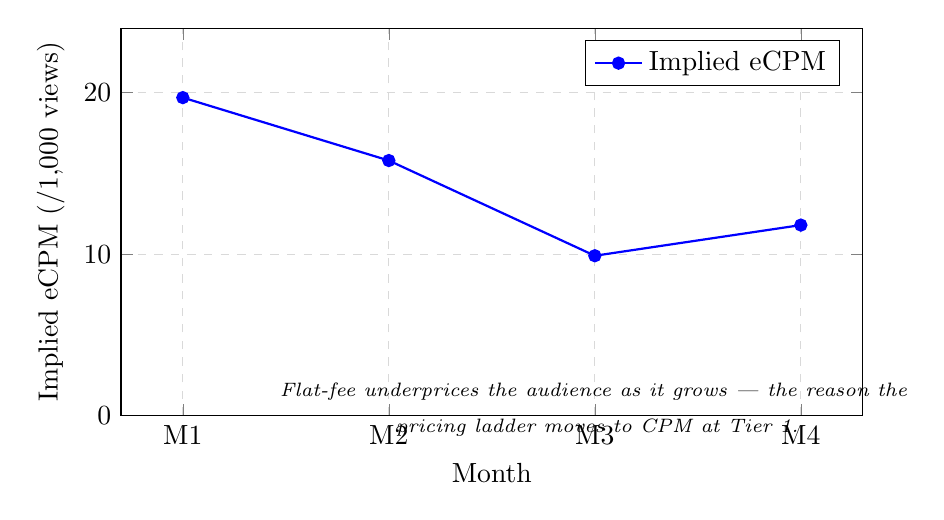
\begin{tikzpicture}
\begin{axis}[
  width=11cm, height=6.5cm,
  xlabel={Month}, ylabel={Implied eCPM (\textrm{\textrupee}/1,000 views)},
  xtick={1,2,3,4}, xticklabels={M1,M2,M3,M4},
  ymin=0, ymax=24,
  legend pos=north east,
  grid=major, grid style={dashed, gray!30},
]
\addplot[mark=*, thick, blue] coordinates {(1,19.7) (2,15.8) (3,9.9) (4,11.8)};
\legend{Implied eCPM, Tier 0}
\end{axis}
\node[font=\scriptsize\itshape, align=left] at (6.0,0.3) {Flat-fee underprices the audience as it grows --- the reason the};
\node[font=\scriptsize\itshape, align=left] at (6.05,-0.15) {pricing ladder moves to CPM at Tier 1.};
\end{tikzpicture}
\caption{Implied-eCPM decay under Tier-0 flat-fee pricing as the active-developer base grows.}
\label{fig:ecpm-decay}
\end{figure}

\section{Months 5--24: three scenarios}
\label{sec:scenarios}

No workbook models past Month 4. The extension below is new planner work --- Tier-0 flat-fee economics held until MASTER-PLAN \S 5.1's Tier-1 trigger (5--10 advertisers signed), then per-advertiser revenue converts to the Tier-1 rate card (\$2--3 CPM India, dev share \(\approx\) \$1--1.5/block \(\approx\) \textrm{\textrupee}94--141 at the locked \textrm{\textrupee}94 FX). The install curve is a planner-constructed S-curve consistent with the \emph{observed} M1--M4 growth rate, not a researched adoption curve. All figures past Month 4 are \textbf{\textit{[Internal assumption --- planner extrapolation]}}.

\begin{table}[htbp]
\centering
\caption{Worst-case scenario, M4--M24}
\label{tab:scenario-worst}
\small
\begin{tabular}{lrrrrrr}
\toprule
& \textbf{M4 (locked)} & \textbf{M6} & \textbf{M9} & \textbf{M12} & \textbf{M18} & \textbf{M24} \\
\midrule
Installs (cum.) & 500 & 550 & 600 & 650 & \textasciitilde 700 & \textasciitilde 700 \\
Advertisers & 3 & 2 (no renewal) & 1 & 1 & 1 & 1 \\
Revenue (\textrm{\textrupee}/mo) & 45,000 & 30,000 & 15,000 & 15,000 & 15,000 & 15,000 \\
Tier & 0 & 0 & 0 & 0 & 0 & 0 \\
Net profit (\textrm{\textrupee}/mo) & 17,320 & \textasciitilde 9,800 & \textasciitilde 5,000 & \textasciitilde 5,000 & \textasciitilde 5,000 & \textasciitilde 5,000 \\
\bottomrule
\end{tabular}
\end{table}

\begin{table}[htbp]
\centering
\caption{Likely-case scenario, M4--M24}
\label{tab:scenario-likely}
\small
\begin{tabular}{lrrrrrr}
\toprule
& \textbf{M4 (locked)} & \textbf{M6} & \textbf{M9} & \textbf{M12} & \textbf{M18} & \textbf{M24} \\
\midrule
Installs (cum.) & 500 & 900 & 1,600 & 2,800 & \textasciitilde 5,500 & \textasciitilde 9,000 \\
Advertisers & 3 & 4 & 6 (Tier 1 activates) & 8 & 8--10 & 10 \\
Revenue (\textrm{\textrupee}/mo) & 45,000 & 60,000 & \textasciitilde 95,000 & \textasciitilde 165,000 & \textasciitilde 150,000--250,000 & \textasciitilde 150,000--300,000 \\
Net profit (\textrm{\textrupee}/mo) & 17,320 & \textasciitilde 28,000 & \textasciitilde 42,000 & \textasciitilde 78,000 & \textasciitilde 150,000 & \textasciitilde 280,000 \\
Cumulative net (\textrm{\textrupee}) & 39,520 & \textasciitilde 110,000 & \textasciitilde 280,000 & \textasciitilde 650,000 & \textasciitilde 1,500,000 & \textasciitilde 3,200,000 \\
\bottomrule
\end{tabular}
\end{table}

\begin{table}[htbp]
\centering
\caption{Best-case scenario, M4--M24}
\label{tab:scenario-best}
\small
\begin{tabular}{lrrrrrr}
\toprule
& \textbf{M4 (locked)} & \textbf{M6} & \textbf{M9} & \textbf{M12} & \textbf{M18} & \textbf{M24} \\
\midrule
Installs (cum.) & 500 & 1,500 & 4,000 & 8,000 & \textasciitilde 16,000 & \textasciitilde 30,000 \\
Advertisers & 3 & 6 & 10 & 15 & 18 & 20+ \\
Revenue (\textrm{\textrupee}/mo) & 45,000 & 110,000 & \textasciitilde 300,000 & \textasciitilde 620,000 & \textasciitilde 850,000 & \textasciitilde 1,600,000 \\
Net profit (\textrm{\textrupee}/mo) & 17,320 & \textasciitilde 70,000 & \textasciitilde 210,000 & \textasciitilde 450,000 & \textasciitilde 850,000 & \textasciitilde 1,600,000 \\
Cumulative net (\textrm{\textrupee}) & 39,520 & \textasciitilde 230,000 & \textasciitilde 900,000 & \textasciitilde 2,500,000 & \textasciitilde 6,500,000 & \textasciitilde 14,000,000 \\
\bottomrule
\end{tabular}
\end{table}

\textbf{Reconciliation note on the two source models' M24 figures.} The TAM-research scenario table and the planner financial extension were built independently and converge closely for the \textbf{Likely} case (both land \textasciitilde \textrm{\textrupee}150k--300k/mo, \textasciitilde 5,000--9,000 installs at M24). They diverge on the \textbf{Best} case: the TAM research caps best-case M24 at \textasciitilde \textrm{\textrupee}500k--900k/mo (12,000--20,000 installs), while the planner extension runs to \textasciitilde \textrm{\textrupee}1.6M/mo (30,000 installs). We present the planner figures as the upper rail and the TAM-research figures as a more conservative best case, and treat the \emph{Likely} convergence as the load-bearing number. The Best-case divergence is two compounding layers of unverified assumption and should be read as a thought experiment, not diligence.

\begin{figure}[htbp]
\centering
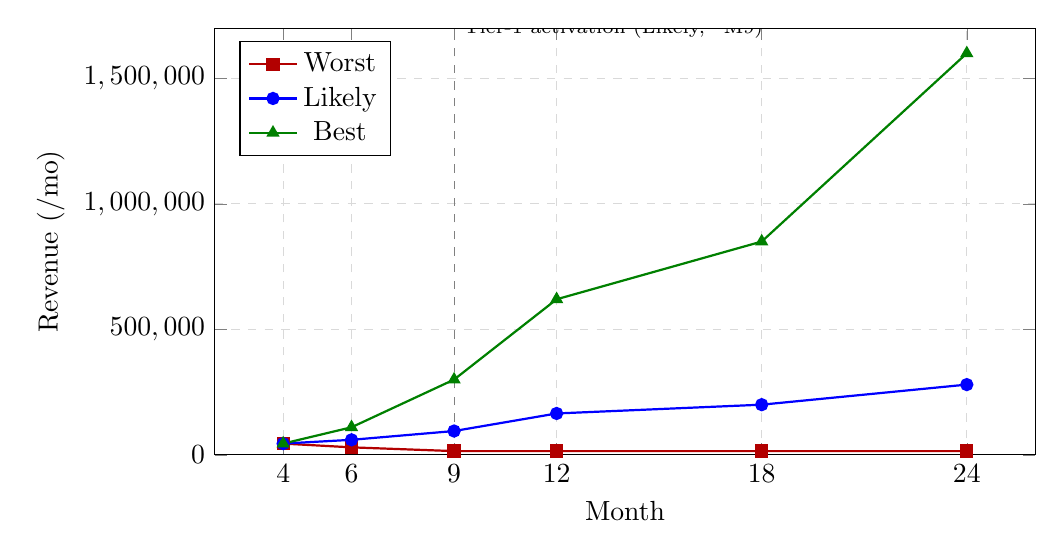
\begin{tikzpicture}
\begin{axis}[
  width=12cm, height=7cm,
  xlabel={Month}, ylabel={Revenue (\textrm{\textrupee}/mo)},
  xtick={4,6,9,12,18,24},
  ymin=0, ymax=1700000,
  legend pos=north west,
  grid=major, grid style={dashed, gray!30},
  scaled y ticks=false,
  yticklabel style={/pgf/number format/.cd, fixed, fixed zerofill=false, 1000 sep={,}},
]
\addplot[mark=square*, thick, red!70!black] coordinates {(4,45000) (6,30000) (9,15000) (12,15000) (18,15000) (24,15000)};
\addplot[mark=*, thick, blue] coordinates {(4,45000) (6,60000) (9,95000) (12,165000) (18,200000) (24,280000)};
\addplot[mark=triangle*, thick, green!50!black] coordinates {(4,45000) (6,110000) (9,300000) (12,620000) (18,850000) (24,1600000)};
\draw[dashed, gray] (axis cs:9,0) -- (axis cs:9,1700000);
\node[font=\scriptsize, anchor=south west] at (axis cs:9,1620000) {Tier-1 activation (Likely, \textasciitilde M9)};
\legend{Worst, Likely, Best}
\end{axis}
\end{tikzpicture}
\caption{24-month revenue scenarios. Tier 2 (real-time auction, 5,000+ DAU threshold) is not reached in any scenario through M12.}
\label{fig:revenue-scenarios}
\end{figure}

\begin{figure}[htbp]
\centering
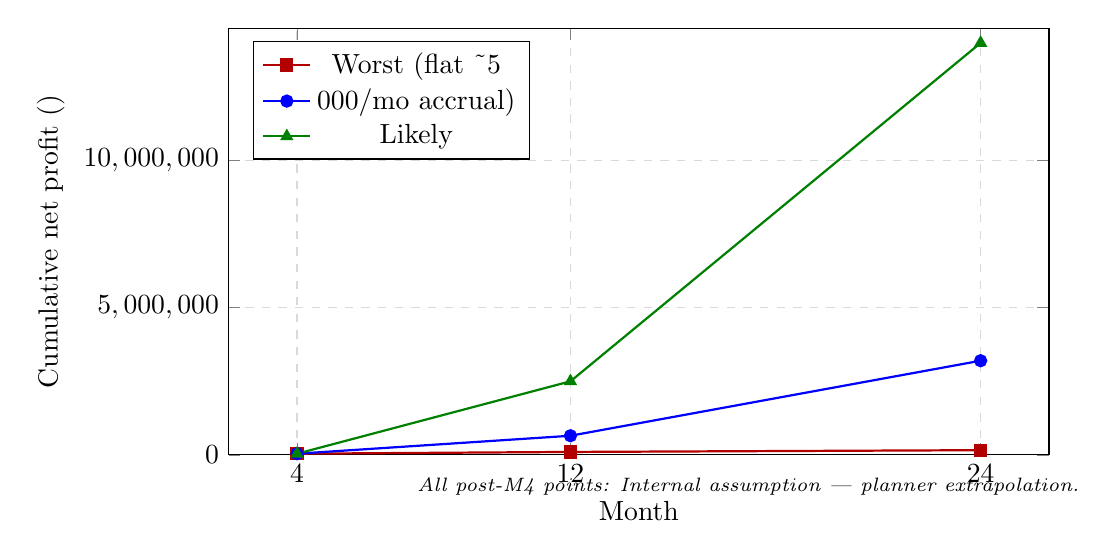
\begin{tikzpicture}
\begin{axis}[
  width=12cm, height=7cm,
  xlabel={Month}, ylabel={Cumulative net profit (\textrm{\textrupee})},
  xtick={4,12,24},
  ymin=0, ymax=14500000,
  legend pos=north west,
  grid=major, grid style={dashed, gray!30},
  scaled y ticks=false,
  yticklabel style={/pgf/number format/.cd, fixed, fixed zerofill=false, 1000 sep={,}},
]
\addplot[mark=square*, thick, red!70!black] coordinates {(4,39520) (12,99520) (24,159520)};
\addplot[mark=*, thick, blue] coordinates {(4,39520) (12,650000) (24,3200000)};
\addplot[mark=triangle*, thick, green!50!black] coordinates {(4,39520) (12,2500000) (24,14000000)};
\legend{Worst (flat \textasciitilde\textrm{\textrupee}5,000/mo accrual), Likely, Best}
\end{axis}
\node[font=\scriptsize\itshape, align=left] at (6.6,-0.4) {All post-M4 points: Internal assumption --- planner extrapolation.};
\end{tikzpicture}
\caption{Cumulative net profit by scenario, M4--M24.}
\label{fig:cumulative-net}
\end{figure}

\subsection*{Reading the scenarios}

\textbf{Worst case is not ``zero'' --- it is ``stuck at Tier 0 indefinitely,''} which is still cash-flow-positive against the \textasciitilde \textrm{\textrupee}5,000/mo cost base. This is precisely the ``stop and rethink'' branch MASTER-PLAN \S 8.3 defines: if \(\geq\) 2 advertisers don't renew, the plan says stop, not keep projecting. Shown for completeness, not as a target.

\textbf{Likely case} assumes the gate clears and at least one of the two structural bottlenecks (advertiser sales; retention past novelty) resolves favorably --- not both.

\textbf{Best case} requires both to resolve favorably \emph{and} requires IdleAds' 70\%/90\%-goal rev-share not to meaningfully erode Devorix's developer supply against the locked 50/50.

\textbf{The single most important caveat:} even the BEST case stays inside the Tier 0/Tier 1 hybrid pricing regime through Month 12 --- 8,000 installs is still well short of the 5,000+ DAU threshold for Tier 2 (real-time auction). Tier 2 is realistically an 18--24 month conversation under every scenario. Two real-world facts puncture any naive continuation of these curves: (1) IdleAds already offers a 70\% dev rev-share versus the locked 50\% --- dev-supply competition is a real risk to the install curve at this horizon, not a footnote (flagged for monitoring, \emph{not} a reopening of the locked 50/50 decision); (2) the category is 2.5 weeks old with zero proven advertiser retention anywhere --- a 24-month projection here is closer to a thought experiment than a forecast.

\section{Unit economics}
\label{sec:unit-economics}

\begin{table}[htbp]
\centering
\caption{Unit economics}
\label{tab:unit-economics}
\small
\begin{tabular}{p{4.0cm}p{3.4cm}p{2.6cm}p{3.0cm}}
\toprule
\textbf{Metric} & \textbf{Value} & \textbf{Source} & \textbf{Label / Note} \\
\midrule
Revenue / active dev / month (Tier 0, M4) & \textrm{\textrupee}225 gross (\textrm{\textrupee}45,000 \(\div\) 200) & REALISTIC \texttt{Plan\_4mo\_FlatDeals} & Dev share = \textrm{\textrupee}112.50 \\
Dev payout / active dev / month (Tier 0, M1--M4) & \textrm{\textrupee}93.75--\textrm{\textrupee}187.50 & Same & \textbf{Non-monotonic} --- drops M1\(\to\)M3 (\textrm{\textrupee}187.50\(\to\)\textrm{\textrupee}93.75) as installs outpace flat-fee advertiser revenue, recovers M4 \\
Revenue / advertiser / month (Tier 0) & \textrm{\textrupee}15,000 flat & MASTER-PLAN \S 5.1--5.2; all 3 workbooks & \textbf{Locked} --- the number to quote in pitches, not CPM-derived \\
Revenue / advertiser / month (Tier 1) & \$2--3 CPM-equiv.\ India; depends on audience at activation & MASTER-PLAN \S 5.4 & \textit{[Internal assumption -- revisit once Tier 1 has real fill data]} (founder's tag) \\
Contribution margin per \textrm{\textrupee} revenue & 50\% (= dev rev share), before fixed costs & Decision \#11; all workbooks & Payout txn cost (\textrm{\textrupee}3--4/txn, RazorpayX) \(\approx\) \textrm{\textrupee}180/mo at M4 = 0.4\% of revenue, rounds to \textasciitilde 0 \\
Fixed costs / month (Tier 0 era) & \textasciitilde \textrm{\textrupee}5,000--5,200 (infra \textrm{\textrupee}3,000 + misc \textrm{\textrupee}2,000 + payout fees) & REALISTIC & Founder salary = \textrm{\textrupee}0 (sweat equity) --- flag to investors: not fully-loaded \\
Tier 0 \(\to\) 1 step-change & From a share of flat \textrm{\textrupee}15,000 (no per-impression accounting) to \$1--1.5/block (\textrm{\textrupee}94--141) priced per filled impression & MASTER-PLAN \S 5.1, \S 5.4 & A pricing-\emph{model} change, not just volume; requires the block-serving engine to exist (\texttt{00-MVP-spec.md} \S 4, not yet built) \\
Steady-state per-dev ceiling (sanity check, NOT the plan) & \textrm{\textrupee}151.36/dev/month at \$2 eCPM, 100\% fill & \texttt{devorix-financial-model.xlsx} \texttt{Scenarios} & \textbf{Superseded model} --- upper-bound only; 100\% fill unrealistic at any modeled horizon \\
Reality-check floor (why CPM-only fails at small scale) & 500 installs / 200 active / 15\% fill \(\to\) gross \textrm{\textrupee}4,990/mo, dev share \textrm{\textrupee}2,495/mo total (\(\approx\) \textrm{\textrupee}12.47/active dev/mo) & REALISTIC \texttt{Reality\_Check\_CPM} & The workbook's own justification for why Tier 0 must be flat-fee --- load-bearing for MASTER-PLAN \S 5's whole pricing architecture \\
\bottomrule
\end{tabular}
\end{table}

\textbf{Headline unit-economics read:} at Tier 0, each advertiser is a clean \textrm{\textrupee}15,000/mo at 50\% contribution margin, and the business is cash-positive from Month 1 because costs are \textasciitilde \textrm{\textrupee}5,000/mo. The non-monotonic per-dev payout is the clearest single signal that flat-fee pricing is a deliberate early-stage choice (sellable at small scale) that underprices the audience as it grows --- which is exactly why the ladder moves to CPM at Tier 1.

\section{Sensitivity: which assumptions move the model most}
\label{sec:sensitivity}

Ranked by modeled swing, drawn from the workbooks' own sensitivity sheets plus the M4--M24 extension.

\begin{table}[htbp]
\centering
\caption{Sensitivity ranking}
\label{tab:sensitivity}
\small
\begin{tabular}{cp{3.2cm}p{2.6cm}p{4.4cm}p{2.4cm}}
\toprule
\textbf{Rank} & \textbf{Assumption} & \textbf{Range tested} & \textbf{Effect on monthly platform margin} & \textbf{Source} \\
\midrule
1 & \textbf{Fill rate} (\% of impressions sold to a paying advertiser) & 5\% \(\to\) 100\% & At 200 active devs: \textrm{\textrupee}9,029 \(\to\) \textrm{\textrupee}180,576 gross/mo --- a \textbf{20\(\times\)} swing from this variable alone & v3 \texttt{Platform\_Scale} --- called ``THE constraint'' \\
2 & \textbf{Active-developer count} (install\(\to\)WAU funnel) & 50 \(\to\) 500 devs & At fixed 30\% fill: \textrm{\textrupee}27,086 \(\to\) \textrm{\textrupee}270,864 gross/mo --- a \textbf{10\(\times\)} swing & v3 \texttt{Platform\_Scale} --- compounds multiplicatively with rank 1 \\
3 & \textbf{Pricing-model choice} (flat vs.\ CPM) at same audience & Flat \textrm{\textrupee}15,000/advertiser vs.\ CPM & Same 3.8M views/mo: flat = \textrm{\textrupee}30,000 (eCPM \textrm{\textrupee}7.89) vs.\ CPM = \textrm{\textrupee}108,346 (eCPM \textrm{\textrupee}28.50) --- a \textbf{3.6\(\times\)} difference for identical usage & v3 \texttt{CPM\_vs\_FlatDeal} \\
4 & \textbf{eCPM level} (secondary) & \$0.8 \(\to\) \$5.0 & At 10,000 devs, full fill: \textrm{\textrupee}6.05L \(\to\) \textrm{\textrupee}37.84L/mo --- \textbf{6.25\(\times\)} & \texttt{devorix-financial-model.xlsx} \texttt{Scenarios} --- superseded \textrm{\textrupee}86 FX/CPM-only; directionally valid \\
5 & \textbf{Going global} (\% foreign users, secondary) & 0\% \(\to\) 20\% foreign & Same 200 active base: India-only \textrm{\textrupee}108,346/mo vs.\ blended \textrm{\textrupee}194,338/mo --- a \textbf{1.79\(\times\)} uplift & v3 \texttt{Global\_Blended} --- gated behind MASTER-PLAN \S 8.1's ``Global = Phase 2'' \\
\bottomrule
\end{tabular}
\end{table}

\begin{figure}[htbp]
\centering
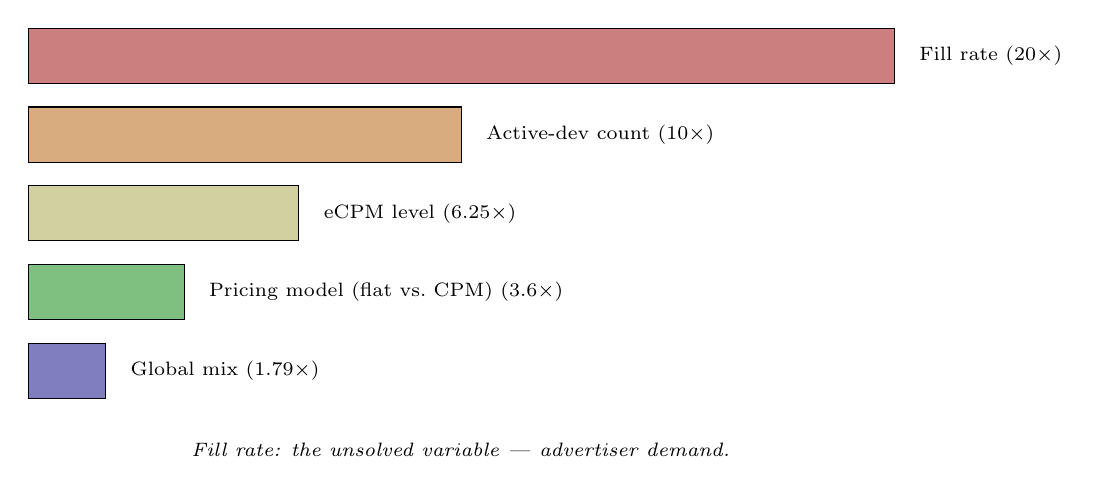
\begin{tikzpicture}[every node/.style={font=\small}]
\def\scl{0.55}
\foreach \rank/\lbl/\val/\col in {%
  1/{Fill rate}/20/red!60!black,%
  2/{Active-dev count}/10/orange!70!black,%
  3/{eCPM level}/6.25/yellow!60!black,%
  4/{Pricing model (flat vs.\ CPM)}/3.6/green!50!black,%
  5/{Global mix}/1.79/blue!50!black%
} {
  \pgfmathsetmacro{\ypos}{-(\rank-1)*1.0}
  \node[draw, fill=\col, fill opacity=0.5, draw opacity=1, minimum height=0.7cm, minimum width=\val*\scl cm, anchor=west] at (0,\ypos) {};
  \node[anchor=west, font=\scriptsize] at (\val*\scl+0.2,\ypos) {\lbl\ (\val\(\times\))};
}
\node[font=\scriptsize\itshape, align=left] at (5.5,-5.0) {Fill rate: the unsolved variable --- advertiser demand.};
\end{tikzpicture}
\caption{Sensitivity tornado: modeled swing in monthly platform margin by assumption.}
\label{fig:sensitivity-tornado}
\end{figure}

\textbf{Why this matters for the risk framing:} the top two levers --- fill rate and active-dev count --- are both downstream of the same root cause MASTER-PLAN names as the central risk: \textbf{advertiser demand, not developer supply, is the bottleneck}. Fill rate is literally ``can we find advertisers to buy inventory we already have.'' The model is far more sensitive to a variable nobody has solved yet (fill rate) than to a comparatively tractable one (install growth). The PRD's financial model should lead with this, not bury it. The CPM rate and 50/50 split are locked and not modeled as variables --- but for the risk section: IdleAds' 70\%/90\%-goal split is an advertiser-supply-indifferent lever a competitor can pull that Devorix has chosen not to. A competitive sensitivity worth flagging, not a reopening of the locked decision.

\section{Open numeric gaps for further research (financial)}

\begin{enumerate}
  \item Realistic \textbf{fill-rate trajectory} month-over-month once \(\geq\) 1 advertiser is signed --- rank \#1 sensitivity, currently a blue-cell assumption in every workbook (5\%\(\to\)100\% original, 15\% REALISTIC, 30\% v3) with no empirical basis. Highest-value number to replace with real data after the sprint.
  \item \textbf{Week-4 developer retention} --- a \S 8.3 go/no-go condition; no workbook models churn, only cumulative installs.
  \item \textbf{Ring 1 + Ring 2 total addressable ad budget} (the Tier-1/Tier-2 revenue ceiling) --- unsized anywhere.
  \item \textbf{India-specific dev-tool-marketer ad spend} --- all current comps (Carbon Ads, EthicalAds, Stack Overflow Ads) are US/global; Devorix is India-first.
\end{enumerate}

\bigskip
\noindent\textit{Near-term locked inputs (Months 1--4, Section~\ref{sec:months-1-4}) are audited and load-bearing for the funding ask. All 12--24 month figures (Section~\ref{sec:scenarios}, and rows 4--5 of Section~\ref{sec:sensitivity}) are labeled Internal assumption / vision-context and must not be presented to investors as derived from the workbooks --- only Months 1--4 are.}
